\documentclass[10pt]{beamer}

\usetheme{Madrid}
\usecolortheme{default}

\usepackage{graphicx}
\usepackage{booktabs}
\usepackage{amsmath}
\usepackage{subcaption}
\usepackage{hyperref}
\usepackage{xcolor}

\title[Portuguese Tourism Forecasting]{Time Series Modeling and Forecasting of Monthly Tourist Arrivals in Portugal}
\subtitle{Specialized Accommodation Sector Analysis\\https://github.com/s126784/series-temporais}
\author{Oleksandr Solovei (\#126784)}
\date{June 16, 2025}

\begin{document}

\begin{frame}
\titlepage
\end{frame}

\begin{frame}{Outline}
\tableofcontents
\end{frame}

\section{Introduction \& Objectives}

\begin{frame}{Project Overview}
\begin{columns}
\begin{column}{0.55\textwidth}
\begin{itemize}
\item \textbf{Dataset}: 84 monthly observations (2017--2023)
\item \textbf{Source}: INE -- Portugal's National Statistics Office
\item \textbf{Methodology}: Box \& Jenkins SARIMA modeling (validated with ETS and ARCH diagnostics)
\item \textbf{Challenge}: COVID-19 disruption (2020--2021)
\item \textbf{Goal}: Methodological comparison and uncertainty quantification
\item \textbf{Importance}: Tourism industry strategic planning
\end{itemize}

\end{column}

\begin{column}{0.45\textwidth}
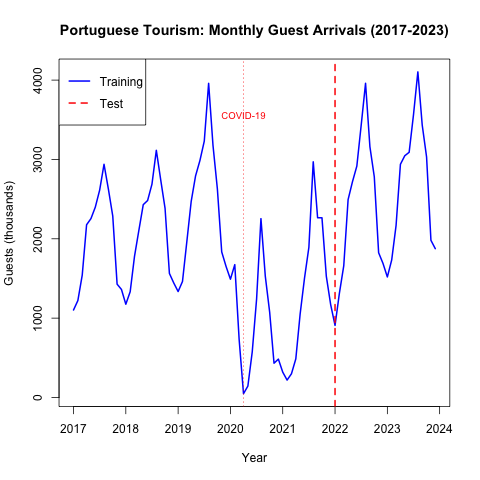
\includegraphics[width=\textwidth,keepaspectratio]{plots/monthly-guest-arrivals.png}
\end{column}
\end{columns}
\end{frame}

% \begin{frame}{Project Importance}
% \begin{columns}
% \begin{column}{0.5\textwidth}
% \textbf{Business Applications}
% \begin{itemize}
% \item Strategic resource allocation
% \item Capacity planning for peak seasons
% \item Informed marketing and policy design
% \item Investment evaluation in tourism infrastructure
% \end{itemize}

% \vspace{0.4cm}
% \textbf{Technical Contribution}
% \begin{itemize}
% \item Rigorous SARIMA vs ETS comparison
% \item Post-COVID forecasting challenges analysis
% \item Uncertainty quantification methodology
% \end{itemize}
% \end{column}

% \begin{column}{0.5\textwidth}
% 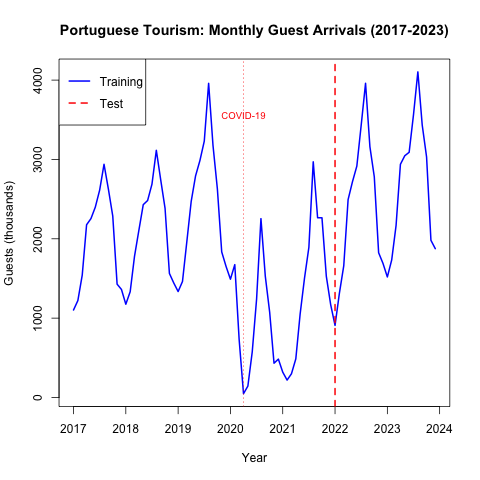
\includegraphics[width=\textwidth,height=0.8\textheight,keepaspectratio]{plots/monthly-guest-arrivals.png}
% \end{column}
% \end{columns}
% \end{frame}

\section{Data Analysis}

\begin{frame}{Dataset Overview}
\begin{columns}
\begin{column}{0.45\textwidth}
\textbf{Key Statistics:}
\begin{itemize}
\item \textbf{Period}: Jan 2017 -- Dec 2023
\item \textbf{Split}: Train (2017--2021), Test (2022--2023)
\item \textbf{Volatility}: CV = 47.8\%
\end{itemize}

\vspace{0.3cm}
\textbf{Data Quality:}
\begin{itemize}
\item No missing values
\item Consistent monthly reporting
\item Clear seasonal patterns
\item Structural break identified (2020)
\end{itemize}

\end{column}

\begin{column}{0.55\textwidth}
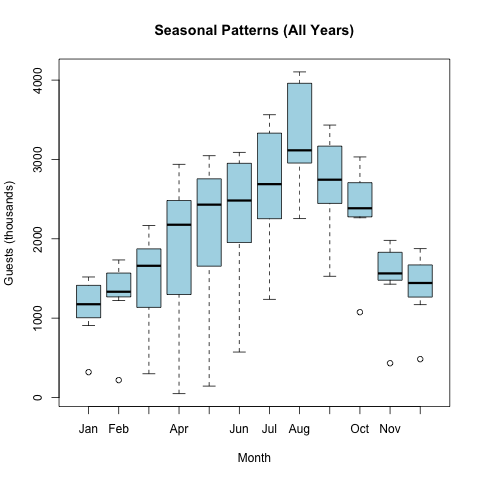
\includegraphics[width=\textwidth,height=0.85\textheight,keepaspectratio]{plots/seasonal-patterns.png}
\end{column}
\end{columns}
\end{frame}

\begin{frame}{Seasonal Patterns}
\begin{columns}
\begin{column}{0.45\textwidth}
\textbf{Observations:}
\begin{itemize}
\item Strong annual seasonality
\item August consistently peaks
\item Repeatable within-year pattern
\item Summer season dominance
\end{itemize}

\vspace{0.3cm}
\textbf{Pattern Analysis:}
\begin{itemize}
\item Q3 accounts for 40\% of annual arrivals
\item Peak-to-trough ratio ≈ 3.4:1
\item Winter months show lowest variability
\item Seasonal patterns remain stable post-COVID
\end{itemize}
\end{column}

\begin{column}{0.55\textwidth}
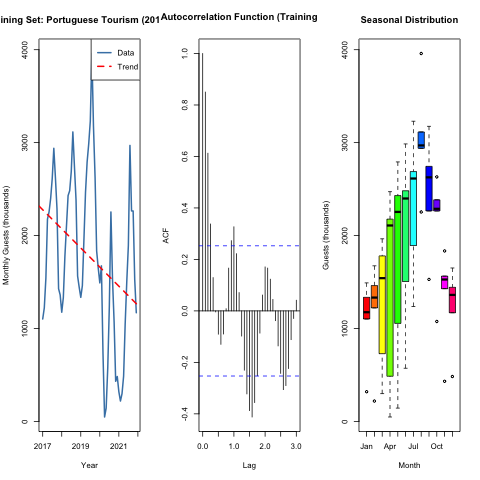
\includegraphics[width=\textwidth,height=0.85\textheight,keepaspectratio]{plots/exploratory-analysis.png}
\end{column}
\end{columns}
\end{frame}

\begin{frame}{STL Decomposition}
\begin{columns}
\begin{column}{0.45\textwidth}
\textbf{STL Components:}
\begin{itemize}
\item \textbf{Seasonality}: Stable and dominant
\item \textbf{Trend}: Disrupted by COVID-19
\item \textbf{Residual}: Minor irregular component
\end{itemize}

\vspace{0.3cm}
\textbf{Key Findings:}
\begin{itemize}
\item Seasonal amplitude relatively constant
\item Trend shows clear structural break in 2020
\item Low residual variance indicates good decomposition
\item Recovery pattern visible from 2021
\end{itemize}
\end{column}

\begin{column}{0.55\textwidth}
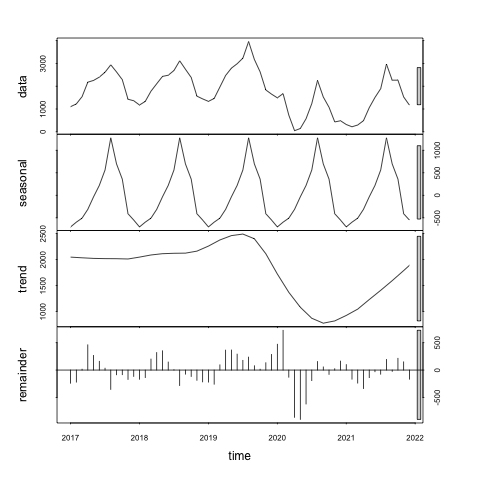
\includegraphics[width=\textwidth,height=0.85\textheight,keepaspectratio]{plots/decomposition-stl.png}
\end{column}
\end{columns}
\end{frame}

\begin{frame}{COVID-19 as Structural Break}
\begin{columns}
\begin{column}{0.45\textwidth}
\textbf{Structural Break Evidence:}
\begin{itemize}
\item \textbf{2020 collapse:} -60.4\% vs 2019
\item \textbf{Slow recovery:} 2021 still -45.8\% below 2019
\item \textbf{Volatility surge:} CV increased to 47.8\%
\item \textbf{Regime change:} New post-COVID baseline
\end{itemize}

\vspace{0.3cm}
\textbf{Impact on Models:}
\begin{itemize}
\item \textbf{SARIMA:} Assumes stable parameters
\item \textbf{ETS:} Adaptive smoothing parameters
\end{itemize}
\end{column}

\begin{column}{0.55\textwidth}
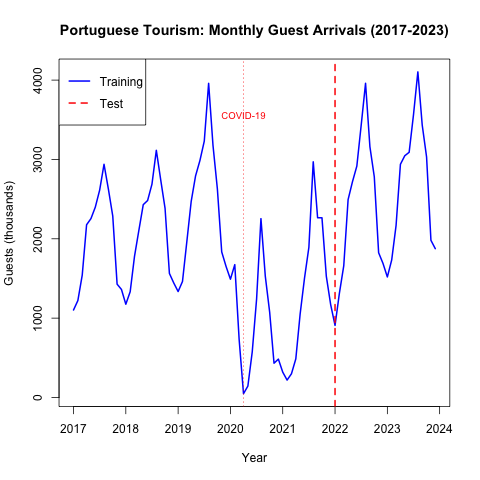
\includegraphics[width=\textwidth,height=0.85\textheight,keepaspectratio]{plots/monthly-guest-arrivals.png}
\end{column}
\end{columns}

\end{frame}

\section{Methodology}

\begin{frame}{Stationarity Analysis}
\begin{columns}
\begin{column}{0.45\textwidth}
\textbf{Preprocessing Steps:}
\begin{itemize}
\item Box-Cox test: $\lambda \approx 1$ (no transformation needed)
\item Seasonal differencing ($D=1$) applied
\item Regular differencing not required ($d=0$)
\end{itemize}

\vspace{0.3cm}
\textbf{Stationarity Tests:}
\begin{itemize}
\item Original series ADF: p = 0.097 (marginally non-stationary)
\item After seasonal diff: p = 0.748 (stationary)

\end{itemize}
\end{column}

\begin{column}{0.55\textwidth}
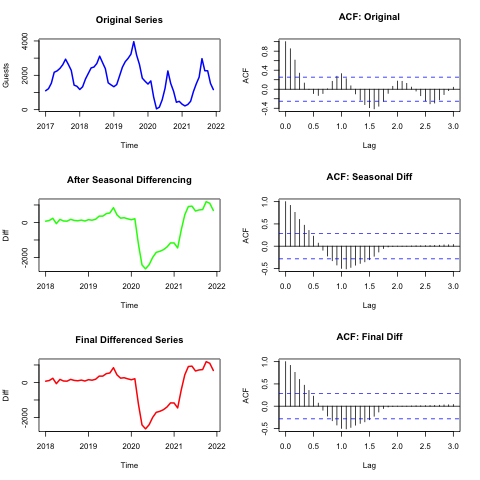
\includegraphics[width=\textwidth,height=0.85\textheight,keepaspectratio]{plots/dif-analysis.png}
\end{column}
\end{columns}
\end{frame}

\begin{frame}{Model Identification}
\begin{columns}
\begin{column}{0.45\textwidth}
\textbf{SARIMA Grid Search:}
\begin{itemize}
\item Parameters: $p,q \in \{0,1,2,3\}$
\item Seasonal: $P,Q \in \{0,1,2\}$
\item Fixed: $s=12$, $D=1$, $d=0$
\item Total models evaluated: 47
\end{itemize}

\vspace{0.3cm}
\textbf{Selection Criteria:}
\begin{itemize}
\item AIC$_c$ and BIC comparison
\item Ljung-Box residual diagnostics
\item Parameter significance tests
\item Out-of-sample validation
\end{itemize}
\end{column}

\begin{column}{0.55\textwidth}
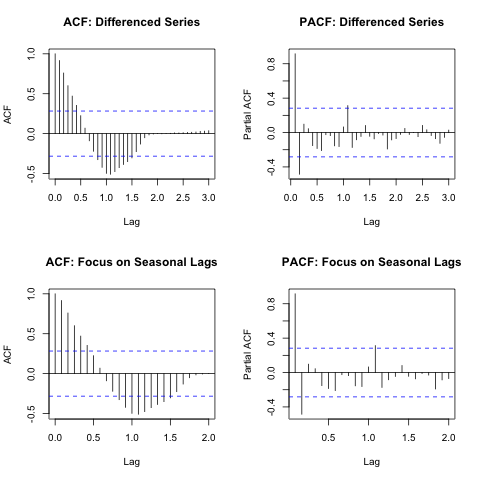
\includegraphics[width=\textwidth,height=0.85\textheight,keepaspectratio]{plots/model-identification.png}
\end{column}
\end{columns}
\end{frame}

\section{Model Selection \& Diagnostics}

\begin{frame}{Top SARIMA Candidates}
\begin{table}[h]
\centering
\small
\begin{tabular}{lcccc}
\toprule
\textbf{Model} & AIC$_c$ & BIC & Ljung-Box p & Rank \\
\midrule
(1,0,1)(1,1,0)[12] & \textbf{694.91} & \textbf{701.46} & \textbf{0.806} & 1 \\
(2,0,0)(1,1,0)[12] & 695.16 & 701.71 & 0.482 & 2 \\
(1,0,1)(0,1,1)[12] & 695.75 & 702.31 & 0.840 & 3 \\
\bottomrule
\end{tabular}
\end{table}

\vspace{0.2cm}
\centering{\textbf{Selected:} SARIMA(1,0,1)(1,1,0)[12]}

\vspace{0.2cm}
\textbf{Selection rationale:} Best balance of parsimony, fit quality, and diagnostic performance
\end{frame}

\begin{frame}{Model Equation \& Parameters}
\begin{block}{Equation}
\begin{align*}
(1 - \phi_1 B)(1 - \Phi_1 B^{12})(1 - B^{12})X_t = (1 + \theta_1 B)\varepsilon_t
\end{align*}
\end{block}

\textbf{Estimated Parameters:}
\begin{itemize}
\item $\phi_1 = 0.869$ (SE=0.069, $p<0.001$) -- Strong autoregressive component
\item $\theta_1 = 0.466$ (SE=0.127, $p<0.001$) -- Moving average correction
\item $\Phi_1 = -0.477$ (SE=0.130, $p<0.001$) -- Seasonal autoregression
\item $\sigma^2_\varepsilon = 33.81$ -- Innovation variance
\end{itemize}

\textbf{Interpretation:} Model captures both short-term momentum and seasonal dependencies
\end{frame}

\begin{frame}{Residual Diagnostics}
\begin{columns}
\begin{column}{0.45\textwidth}
\textbf{Diagnostic Results:}
\begin{itemize}
\item \textbf{Ljung-Box}: p = 0.806 (no autocorrelation)
\item \textbf{Jarque-Bera}: p = 0.089 (approximately normal)
\item \textbf{ARCH Test}: No heteroscedasticity
\item \textbf{Parameter significance}: All $p < 0.001$
\end{itemize}

\vspace{0.3cm}
\textbf{Model Adequacy:}
\begin{itemize}
\item Excellent structural diagnostics
\item Low parameter correlation
\item Stable invertible representation
\item Passes all classical tests
\end{itemize}
\end{column}

\begin{column}{0.55\textwidth}
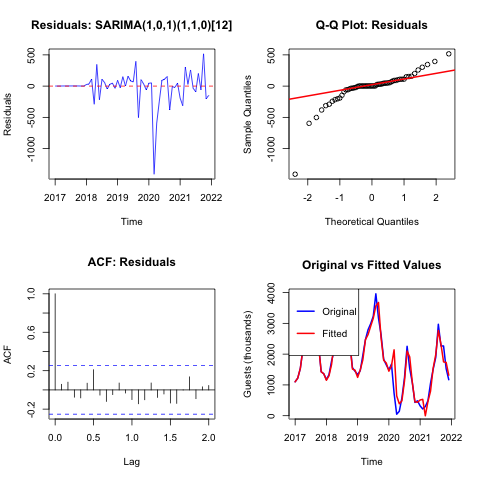
\includegraphics[width=\textwidth,height=0.85\textheight,keepaspectratio]{plots/residuals.png}
\end{column}
\end{columns}
\end{frame}

\section{Validation \& Forecasting}

\begin{frame}{Out-of-Sample Performance}
\begin{columns}
\begin{column}{0.45\textwidth}
\textbf{Test Set Results:}
\begin{itemize}
\item \textbf{RMSE}: 1,468 (thousands)
\item \textbf{MAPE}: \textcolor{red}{51.7\%}
\item \textbf{Directional Accuracy}: 78.3\%
\item \textbf{80\% Coverage}: 41.7\% (target: 80\%)
\item \textbf{95\% Coverage}: 75.0\% (target: 95\%)
\end{itemize}

\vspace{0.3cm}
\textbf{Performance Notes:}
\begin{itemize}
\item Excellent diagnostics ≠ good forecasts
\item Post-COVID volatility challenges
\item Conservative interval coverage
\end{itemize}
\end{column}

\begin{column}{0.55\textwidth}
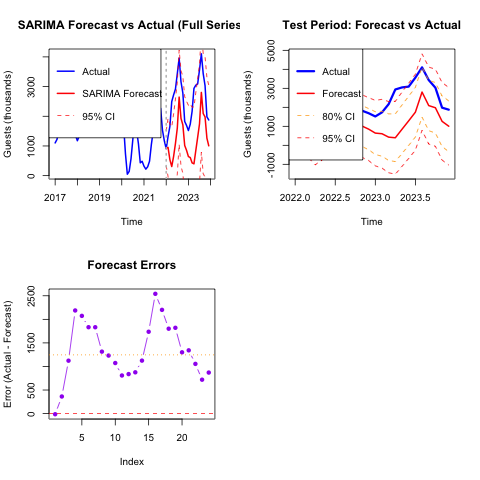
\includegraphics[width=\textwidth,height=0.85\textheight,keepaspectratio]{plots/forecast-vs-actual.png}
\end{column}
\end{columns}
\end{frame}

\begin{frame}{Model Performance Comparison}
\begin{table}[h]
\centering
\small
\begin{tabular}{lcc}
\toprule
Metric & SARIMA & ETS(MAM) \\
\midrule
Training RMSE & 260 & N/A \\
Test RMSE & 1,468 & \textbf{971} \\
MAPE & 51.7\% & \textbf{34.2\%} \\
Directional Accuracy & 78.3\% & N/A \\
AIC$_c$ & \textbf{694.9} & 954.7 \\
Ljung-Box p & \textbf{0.806} & 0.304 \\
\bottomrule
\end{tabular}
\end{table}

\begin{alertblock}{Key Finding}
\textcolor{red}{\textbf{Trade-off:}} SARIMA superior diagnostics, ETS superior forecasting
\end{alertblock}
\end{frame}

\begin{frame}{Model Comparison Summary}
\begin{columns}
\begin{column}{0.45\textwidth}
\begin{block}{SARIMA(1,0,1)(1,1,0)[12]}
\textbf{Strengths:}
\begin{itemize}
\item ✅ Excellent diagnostics (Ljung-Box p=0.806)
\item ✅ All parameters significant (p<0.001)
\item ✅ Better model fit (AICc=694.9)
\item ✅ Theoretical interpretability
\end{itemize}

\textbf{Weaknesses:}
\begin{itemize}
\item ❌ Poor forecasting (MAPE=51.7\%)
\item ❌ Wide confidence intervals
\end{itemize}
\end{block}
\end{column}

\begin{column}{0.45\textwidth}
\begin{block}{ETS(MAM)}
\textbf{Strengths:}
\begin{itemize}
\item ✅ Better forecasting (MAPE=34.2\%)
\item ✅ Superior RMSE \\ (971 vs 1,468)
\item ✅ Adaptive to structural changes
\item ✅ More robust post-COVID
\end{itemize}

\textbf{Weaknesses:}
\begin{itemize}
\item ❌ Higher AICc \\(954.7)
\item ❌ Less theoretical foundation
\end{itemize}
\end{block}
\end{column}
\end{columns}


\end{frame}

\begin{frame}{Forecast Uncertainty Analysis}
\begin{alertblock}{High Uncertainty Environment}
\begin{itemize}
\item \textbf{Year 1:} 95\% CI width = 102.7\% of forecast
\item \textbf{Year 2:} 95\% CI width = 158.7\% of forecast  
\item \textbf{Year 3:} 95\% CI width = 201\% of forecast
\end{itemize}
\end{alertblock}

\textbf{Implications:}
\begin{itemize}
\item Long-term forecasts highly unreliable
\item Focus on seasonal patterns, not absolute levels
\item Scenario planning more valuable than point forecasts
\item Post-COVID structural uncertainty persists
\end{itemize}
\end{frame}



\begin{frame}{2024 Forecast Summary}
\begin{table}[h]
\centering
\footnotesize
\begin{tabular}{lccccc}
\toprule
Month & Forecast & 80\% Low & 80\% High & 95\% Low & 95\% High \\
\midrule
Jan & 1,703 & 1,320 & 2,086 & 1,117 & 2,288 \\
Apr & 3,064 & 2,171 & 3,957 & 1,699 & 4,430 \\
Aug & \textbf{4,226} & 3,136 & 5,315 & 2,560 & 5,892 \\
Dec & 1,921 & 763 & 3,079 & 151 & 3,692 \\
\midrule
Annual & \textbf{33,923} & 22,529 & 45,316 & 16,498 & 51,348 \\
\bottomrule
\end{tabular}
\end{table}

\centering{Units: Thousands of guests}

\begin{alertblock}{Forecast Reliability Warning}
\textbf{2024 vs pre-COVID:} +29.3\% growth, but intervals extremely wide (102.7\% of forecast)
\end{alertblock}
\end{frame}

\begin{frame}{Scenario Analysis \& Planning}
\begin{block}{2024 Planning Scenarios}
\begin{itemize}
\item \textbf{Conservative:} 22.5M guests (-33\% vs expected)
\item \textbf{Expected:} 33.9M guests 
\item \textbf{Optimistic:} 45.3M guests (+34\% vs expected)
\end{itemize}
\end{block}

\textbf{Strategic Recommendations:}
\begin{itemize}
\item Use seasonal patterns for capacity planning
\item Prepare for high volatility scenarios
\item Monitor leading indicators closely
\item Avoid over-reliance on point forecasts
\end{itemize}
\end{frame}

\begin{frame}{Key Research Contributions}
\begin{alertblock}{Methodological Findings}
\textbf{Model diagnostics ≠ Forecast accuracy} in volatile environments
\end{alertblock}

\textbf{Scientific Contributions:}
\begin{itemize}
\item Demonstrated limitations of classical SARIMA in crisis periods
\item Quantified post-COVID forecasting uncertainty in tourism
\item Provided rigorous SARIMA vs ETS comparison methodology
\item Showed importance of out-of-sample validation
\end{itemize}

\textbf{Practical Implications:}
\begin{itemize}
\item Tourism planners: Focus on scenario-based planning
\item Seasonal patterns more reliable than absolute levels
\item Multiple model approaches recommended for volatile periods
\end{itemize}
\end{frame}

\section{Conclusions}

\begin{frame}{Conclusions}
\textbf{Model Performance Assessment:}
\begin{itemize}
\item SARIMA: Excellent structural validity, poor predictive accuracy
\item ETS: Better forecasting performance in volatile environment
\item Both models struggle with post-COVID uncertainty quantification
\end{itemize}

\textbf{Scientific Value:}
\begin{itemize}
\item Highlighted classical time series limitations in crisis periods
\item Demonstrated importance of model comparison beyond diagnostics
\item Provided uncertainty quantification for tourism planning
\end{itemize}

\textbf{Future Research:}
\begin{itemize}
\item Regime-switching models for structural breaks
\item Machine learning ensemble methods  
\item External regressors integration
\end{itemize}

\begin{alertblock}{Key Insight}
In volatile environments, \textbf{structural model validity} and \textbf{predictive accuracy} can diverge significantly
\end{alertblock}
\end{frame}



\begin{frame}{Thank You}
\begin{center}
\Large{\textbf{Questions?}}

\vspace{0.3cm}

https://github.com/s126784/series-temporais\\
\texttt{osolovei@ua.pt}
\end{center}
\end{frame}

\end{document}
